\documentclass[solutions]{esg8012pset} 
  \usepackage{amsmath}
  \usepackage{amssymb}
  \usepackage{enumerate}
  \usepackage{graphicx}
  \usepackage{hyperref}
  %\usepackage{siunitx}
  \providecommand{\uvec}[1]{{\hat{\bf{#1}}}}
  \usepackage{pgf,tikz}
  \usetikzlibrary{arrows}
  \makeatletter
  \newcommand{\interitemtext}[1]{%
    \begin{list}{}
     {\itemindent=0mm\labelsep=0mm
     \labelwidth=0mm\leftmargin=0mm
     \addtolength{\leftmargin}{-\@totalleftmargin}}
      \item #1
    \end{list}
  }
  \makeatother
  \renewcommand{\d}{\,d}
  \providecommand{\norm}[1]{\lVert#1\rVert}
\classname{Physics 8.012} 
\semester{Fall 2010} 
\problemsetnumber{7} 
\date{October 22} 
\duedate{Friday, October 29} 
\readingassignment{Kleppner and Kolenkow, \emph {An Introduction to Mechanics}, Chapter Four} 
\begin{document}
\section*{Problem 1: K\&K 4.21}
\subsection*{Problem}
  An unknown rope of linear mass density $\lambda$ (mass per unit length), is coiled on a smooth horizontal table. On end is pulled straight up with constant speed $v_0$.
  \begin{center}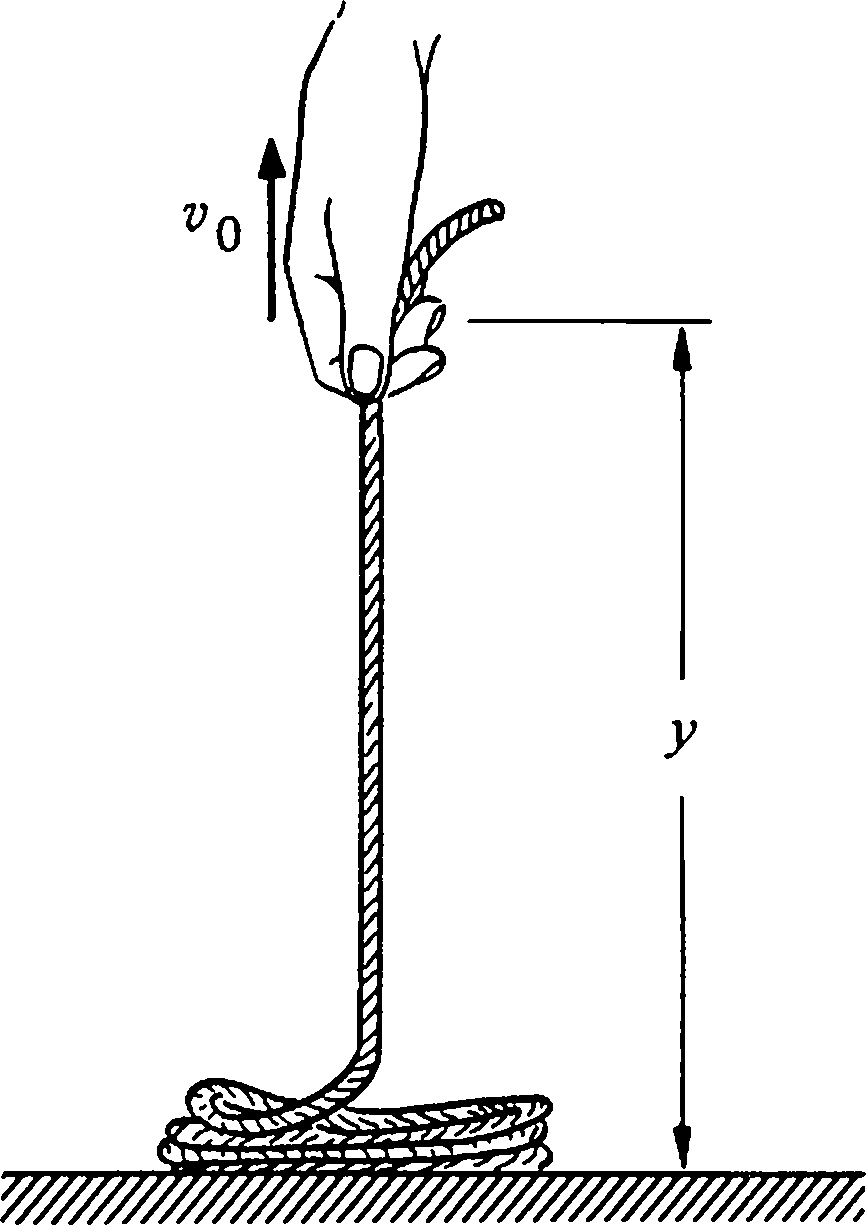
\includegraphics[width=0.2\textwidth]{ps07_1}\end{center}
  \begin{enumerate}[(a)]
  \item Find the force exerted on the end of the rope as a function of the height $y$ of the rope above the table.
    \item Compare the power delivered to the rope with the rate of change of the rope's total mechanical energy. Explain whether they should or should not be equal. Remember that the rope is not a rigid body.
  \end{enumerate}
\subsection*{Solution}
  \begin{enumerate}[a)]
    \item
  \begin{align*}
    F(y) - F_g(y) & = \frac{\d (m v)}{\d t} \\
    F(y) & = \lim_{\Delta t \rightarrow 0} \frac{\lambda (y+\Delta y) v_0 - \lambda y v_0}{\Delta t} + F_g(y) \\
    & = \lim_{\Delta t \rightarrow 0} \frac{\Delta y}{\Delta t} \lambda v_0 + \lambda g y \\
    & = \lambda v_0^2 + \lambda g y
  \end{align*}
    \item \begin{align*}
    K(y) & = \frac{1}{2}\lambda y v_0^2 \\
    U_g(y) & = \int_{0}^y \lambda g z \d z \\
          & = \frac{1}{2}\lambda g y^2 \\
    K(y) + U_g(y) & = \frac{\lambda}{2} y(v_0^2 + g y) \\
    \frac{\d E(y)}{\d t} & = \frac{\lambda}{2} v_0^3 + \lambda g y v_0 \\
    F(y)v_0 & = \lambda v_0^3 + \lambda g y v_0)
    \end{align*} The power delivered to the rope is less than change in mechanical energy per unit time; the rope must heat up.  %be greater than the change in mechanical energy, because some of it goes to gravitational potential energy.  ?
  \end{enumerate}
\section*{Problem 2: K\&K 4.23}
\subsection*{Problem}
  Two superballs are dropped from a height above the ground. The ball on top has a mass $m_1$. The ball on the bottom has a mass $m_2$. Assume that the lower ball collides elastically with the ground. Then as the lower ball starts to move upward, it collides elastically with the upper ball that is still moving downwards. How high will the upper ball rebound in the air? Assume that $m_2 \gg m_1$. Hint: consider this collision from an inertial reference frame that moves upward with the same speed as the lower ball has after it collides with ground. What speed does the upper ball have in this reference frame after it collides with the lower ball?
  \begin{center}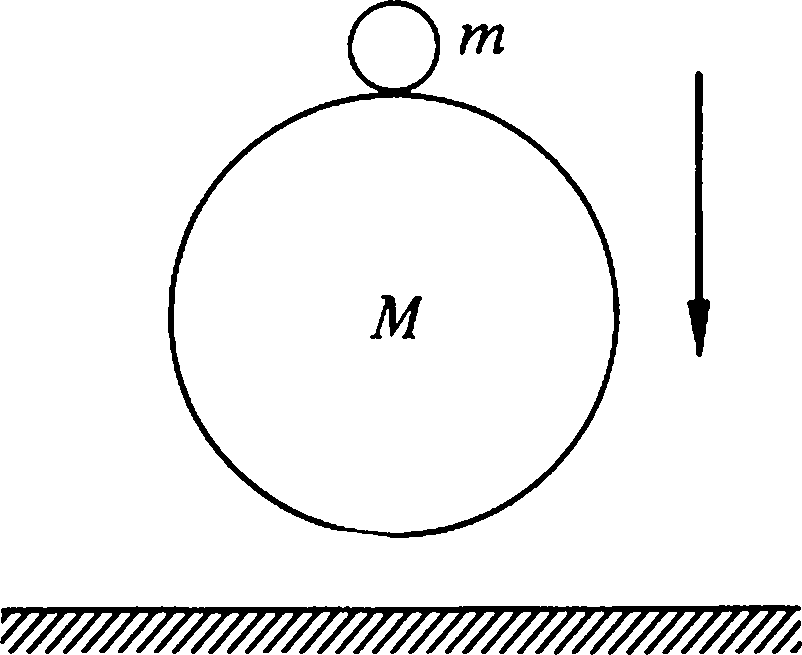
\includegraphics[width=0.25\textwidth]{ps07_2}\end{center}
\subsection*{Solution}
  Let $h_1$ and $h_2$ denote the initial heights of the balls on top and on bottom, respectively.  Suppose that they collide at height $h_3$.  The speed of the bottom ball is $v_{2, i} = \sqrt{2\frac{m_2gh_2 - m_2 g h_3}{m_2}} = \sqrt{2g(h_2 - h_3)}$.  The speed of the top ball is $v_{1, i} = -\sqrt{2g(h_1-h_3)}$.  Suppose that we take the reference frame moving up with speed $v_{2, i}$.  Because the collision is elastic, and suppose that $v_{*, *}' = v_{*, *} - v_{2, i}$ \begin{align*}
    m_1 v_{1,i}' & = m_1 v_{1,f}' + m_2 v_{2,f}' \\
    \frac{1}{2}m_1 v_{1,i}'^2 & = \frac{1}{2}m_1 v_{1,f}'^2 + \frac{1}{2}m_2 v_{2,f}'^2 \\
    \\
    v_{2,f}' & =  \frac{m_1(v_{1,i}' - v_{1,f}')}{m_2} \\
    v_{2,f}'^2 & = \frac{m_1(v_{1,i}'^2 - v_{1,f}'^2)}{m_2} \\
    \\
    v_{2,f}'^2 & = \frac{m_1^2(v_{1,i}' - v_{1,f}')^2}{m_2^2} \\
    v_{2,f}'^2 & = \frac{m_1(v_{1,i}' - v_{1,f}')(v_{1,i}' + v_{1,f}')}{m_2} \\
    \\
    1 & = \frac{m_1(v_{1,i}' + v_{1,f}') m_2^2}{m_2 m_1^2 (v_{1,i}' - v_{1,f}')} \\
      & = \frac{(v_{1,i}' + v_{1,f}') m_2}{m_1 (v_{1,i}' - v_{1,f}')} \\
      & = \frac{m_2}{m_1}\frac{v_{1,i}' + v_{1,f}'}{v_{1,i}' - v_{1,f}'} \\
    m_1(v_{1,i}' - v_{1,f}') & = m_2(v_{1,i}' + v_{1,f}') \\
    v_{1,i}'(m_1 - m_2) & =  v_{1,f}'(m_1 + m_2) \\
    v_{1, f}' & = \frac{m_1 - m_2}{m_1 + m_2}v_{1,i}' \\
    \intertext{Since $v_{1, i}' = v_{1, i} - v_{2, i}$, and $v_{1, f}' = v_{1, f} - v_{2, i}$,}
    v_{1, f} - v_{2, i} & = \frac{m_1 - m_2}{m_1 + m_2}(v_{1, i} - v_{2, i}) \\
    v_{1, f} & = \frac{m_1 - m_2}{m_1 + m_2}(v_{1, i} - v_{2, i}) + v_{2, i} \\
    \intertext{Since $m_2\gg m_1$,}
    v_{1, f} & = (v_{2, i} - v_{1, i}) + v_{2, i} \\
    & = 2v_{2, i} - v_{1, i} \\
    & = 2\sqrt{2g(h_2 - h_3)} + \sqrt{2g(h_1-h_3)}
    \end{align*}
    Then the height, $\sqrt{2g(h_{\text{max}} - h_3)} = 2\sqrt{2g(h_2 - h_3)} + \sqrt{2g(h_1-h_3)}$, so $h_{\text{max}} = 4(h_2 - h_3) + (h_1 - h_3) + 4\sqrt{(h_2 - h_3)(h_1 - h_3)} = 4h_2 + h_1 - 5h_3 + 4\sqrt{(h_2 - h_3)(h_1 - h_3)}$.  Letting $h_3$ go to zero, and $h_1$ and $h_2$ be the same, $h_{\text{max}} = 9h$.
\section*{Problem 3: K\&K 4.25: (Elastic collision in two dimensions)}
\subsection*{Problem}
  A proton makes a head-on collision with an unknown particle at rest. The proton rebounds straight back with $4 / 9$ of its initial kinetic energy. Find the ratio of the mass of the unknown particle to the mass of the proton, assuming that the collision is elastic.
\subsection*{Solution}
  \begin{align*}
  m_p v_{i, p} & = m_p v_{f,p} + m_u v_{f, u} \\
  \frac{1}{2}m_p v_{f, p}^2 & = \frac{4}{9} \frac{1}{2}m_p v_{i, p}^2 \\
  v_{f, p} & = -\frac{2}{3}v_{i, p} \\
  \\
  m_p v_{i, p} & = -m_p \frac{2}{3}v_{i, p} + m_u v_{f, u} \\
  \left(1 + \frac{2}{3}\right)m_p v_{i, p} & = m_u v_{f, u} \\
  \frac{5}{3}m_p v_{i, p} & = m_u v_{f, u} \\
  \frac{5v_{i, p}}{3v_{f, u}} & = \frac{m_u}{m_p} \\
  \\
  \frac{1}{2}m_u v_{f, u}^2 & = \frac{5}{9}\frac{1}{2}m_p v_{i, p}^2 \\
  v_{f, u} & = \frac{\sqrt{5}}{3}\sqrt{\frac{m_p}{m_u}} v_{i, p} \\
  \\
  \frac{m_u}{m_p} & = \frac{3\cdot 5 v_{i, p}}{3\sqrt{5}\sqrt{\frac{m_p}{m_u}} v_{i, p}}  \\
  \sqrt{\frac{m_u}{m_p}} & = \sqrt{5}  \\
  \frac{m_u}{m_p} & = 5
  \end{align*}
\section*{Problem 4: K\&K 4.27}
\subsection*{Problem}
  A particle $A$ of mass $m$ is initially moving in the positive $x$-direction with a speed $v_{A,0}$ and collides elastically with a second particle $B$ of mass $2m$, which is initially at rest.  After the collision the particle $A$ moves with an unknown speed $v_{A,f}$, at an unknown angle $\theta_{A, f}$ with respect to the positive $x$-direction. After the collision, particle $B$ moves with an unknown speed $v_{B, f}$, at an angle $\theta_{2,f} = 45^{\circ}$ with respect to the positive $x$-direction.  Find $\theta_{A, f}$.
  \begin{center}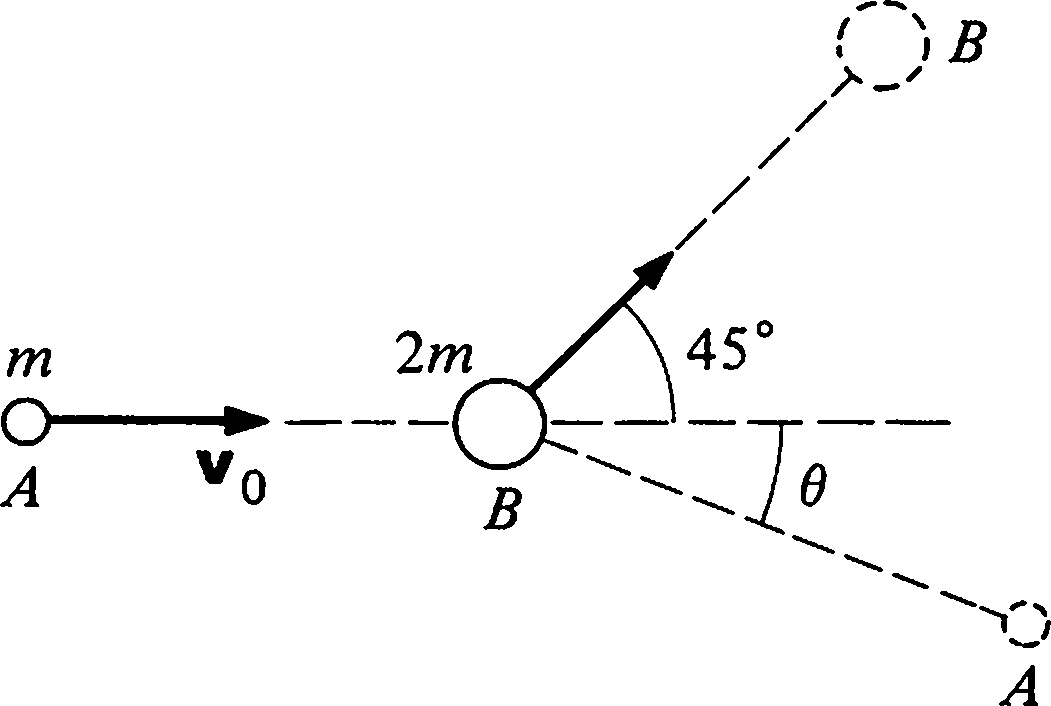
\includegraphics[width=0.3\textwidth]{ps07_3}\end{center}
\subsection*{Solution}
  \begin{align*}
  \hat j& : 0 = m_B v_{B,f}\sin 45^{\circ} - m_A v_{A, f}\sin\theta_{A, f} \\
  \hat i& : m_A v_{A, 0} = m_A v_{A, f}\cos \theta_{A, f} + m_B v_{B, f}\cos 45^{\circ} \\
  K& : \frac{1}{2}m_A v_{A, 0}^2 = \frac{1}{2}m_Av_{A,f}^2 + \frac{1}{2}m_B v_{B, f}^2 \\
  \\
  \hat j& : 0 = \sqrt{2} v_{B,f} - v_{A, f}\sin\theta_{A, f} \\
  \hat i& : v_{A, 0} = v_{A, f}\cos \theta_{A, f} + \sqrt{2}v_{B, f} \\
  K& : v_{A, 0}^2 = v_{A,f}^2 + 2 v_{B, f}^2 \\
  \\
  v_{B,f} & = \frac{v_{A, f}\sin\theta_{A, f}}{\sqrt{2}} \\
  \\
  v_{A, 0} & = v_{A, f}\cos \theta_{A, f} + v_{A, f}\sin\theta_{A, f} \\
  v_{A, 0}^2 & = v_{A,f}^2 + 2 \frac{v_{A, f}^2\sin^2\theta_{A, f}}{2} \\
    & = v_{A,f}^2\left(1 + \sin^2\theta_{A, f}\right) \\
  v_{A, f} & = v_{A, 0}\sqrt{\frac{1}{1 + \sin^2\theta_{A, f}}} \\
  \\
  v_{A, 0} & = v_{A, 0}\sqrt{\frac{1}{1 + \sin^2\theta_{A, f}}}\cos \theta_{A, f} + v_{A, 0}\sqrt{\frac{1}{1 + \sin^2\theta_{A, f}}}\sin\theta_{A, f} \\
  1 & = \sqrt{\frac{1}{1 + \sin^2\theta_{A, f}}}\left(\cos \theta_{A, f} + \sin\theta_{A, f}\right) \\
  \sqrt{1 + \sin^2\theta_{A, f}} & = \cos \theta_{A, f} + \sin\theta_{A, f} \\
  1 + \sin^2\theta_{A, f} & = \cos^2 \theta_{A, f} + \sin^2\theta_{A, f} + 2 \sin \theta_{A, f}\cos \theta_{A, f}\\
  1 + \sin^2\theta_{A, f} & = 1 + 2 \sin \theta_{A, f}\cos \theta_{A, f}\\
  \sin\theta_{A, f} & = 2 \cos \theta_{A, f}\\
  \tan\theta_{A, f} & = 2
  % 0 & = m_B v_{B,f}\sin 45^{\circ} - m_A v_{A, f}\sin\theta_{A, f} \\
  % m_B v_{B,f} & = m_A v_{A, f}\frac{\sin\theta_{A, f}}{\sin 45^{\circ}}
  % \\
  % m_A v_{A, 0}^2 & = m_A v_{A,f}^2 + m_B v_{B, f}^2 \\
  % m_A v_{A, 0}^2 & = m_A v_{A,f}^2 + \frac{\left(m_A v_{A, f}\frac{\sin\theta_{A, f}}{\sin 45^{\circ}}\right)^2}{m_B} \\
  %  & = m_A v_{A,f}^2 + m_A^2 v_{A, f}^2\frac{\frac{\sin^2\theta_{A, f}}{\sin^2 45^{\circ}}}{m_B} \\
  % v_{A, 0}^2 & = v_{A,f}^2\left(1 + \frac{m_A}{m_B}\cdot\frac{\sin^2\theta_{A, f}}{\sin^2 45^{\circ}}\right) \\
  % v_{A,f}^2 & = v_{A, 0}^2\left(1 + \frac{m_A}{m_B}\cdot\frac{\sin^2\theta_{A, f}}{\sin^2 45^{\circ}}\right)^{-1} \\
  % v_{A,f} & = v_{A, 0}\sqrt{1 + \frac{m_A}{m_B}\cdot\frac{\sin^2\theta_{A, f}}{\sin^2 45^{\circ}}}^{-1} \\
  % \\
  % \\
  % \frac{m_A v_{A, f}\sin\theta_{A, f}}{ m_A v_{A, f}\cos\theta_{A, f}} & = \frac{m_B v_{B,f}\sin 45^{\circ}}{m_A v_{A, 0} - m_B v_{B, f}\cos 45^{\circ}} \\
  % \tan\theta_{A, f} & = \frac{m_B}{m_A}\cdot\frac{m_B v_{B,f}\sin 45^{\circ}}{v_{A, 0} - \frac{m_B}{m_A} v_{B, f}\cos 45^{\circ}} \\
  % \tan\theta_{A, f} & = \frac{m_B}{m_A}\cdot\frac{m_A v_{A, f}\frac{\sin\theta_{A, f}}{\sin 45^{\circ}}\sin 45^{\circ}}{v_{A, 0} - \frac{1}{m_A} m_A v_{A, f}\frac{\sin\theta_{A, f}}{\sin 45^{\circ}} \cos 45^{\circ}} \\
  %   & = \frac{m_B}{m_A}\cdot\frac{m_A v_{A, f}\sin\theta_{A, f}}{v_{A, 0} - v_{A, f}\sin\theta_{A, f}\frac{\cos 45^{\circ}}{\sin 45^{\circ}}} \\
  %   & = m_B\cdot\frac{v_{A, f}\sin\theta_{A, f}}{v_{A, 0} - v_{A, f}\sin\theta_{A, f}\frac{\cos 45^{\circ}}{\sin 45^{\circ}}} \\
  %   & = m_B\cdot\frac{v_{A, 0}\sqrt{1 + \frac{m_A}{m_B}\cdot\frac{\sin^2\theta_{A, f}}{\sin^2 45^{\circ}}}^{-1}\sin\theta_{A, f}}{v_{A, 0} - v_{A, 0}\sqrt{1 + \frac{m_A}{m_B}\cdot\frac{\sin^2\theta_{A, f}}{\sin^2 45^{\circ}}}^{-1}\sin\theta_{A, f}\frac{\cos 45^{\circ}}{\sin 45^{\circ}}} \\
  %   & = m_B\cdot\frac{\sin\theta_{A, f}}{\sqrt{1 + \frac{m_A}{m_B}\cdot\frac{\sin^2\theta_{A, f}}{\sin^2 45^{\circ}}} - \sin\theta_{A, f}\frac{\cos 45^{\circ}}{\sin 45^{\circ}}} \\
  %   & = m_B\cdot\frac{1}{\sqrt{\frac{1}{\sin^2\theta_{A, f}} + \frac{m_A}{m_B}\cdot\frac{1}{\sin^2 45^{\circ}}} - \frac{\cos 45^{\circ}}{\sin 45^{\circ}}} \\
  %   \\
  %   \\
  %  & = \frac{m_B}{m_A}\cdot\frac{m_B v_{B,f}\frac{1}{\sqrt{2}}}{v_{A, 0} - \frac{m_B}{m_A} v_{B, f}\frac{1}{\sqrt{2}}} \\
  % \frac{m_B}{m_A}\cdot \frac{-v_{B,f}\sin 45^{\circ}}{v_{A, 0} - v_{A, f}\cos 45^{\circ}} & = \frac{m_A}{m_B}\frac{v_{A, f}\sin\theta_{A, f}}{v_{B, f}\cos\theta_{A, f}} \\
  % \frac{m_B^2}{m_A^2}\cdot \frac{-v_{B,f}\sin 45^{\circ}}{v_{A, 0} - v_{A, f}\cos 45^{\circ}} & = \frac{v_{A, f}}{v_{B, f}}\tan\theta_{A, f} \\
  % \tan\theta_{A, f} & = \frac{v_{B, f}^2}{v_{A, f}}\cdot \frac{m_B^2}{m_A^2}\cdot \frac{-\sin 45^{\circ}}{v_{A, 0} - v_{A, f}\cos 45^{\circ}}  \\
  \end{align*}
\section*{Problem 5: K\&K 4.28}
\subsection*{Problem}
  A thin target of lithium is bombarded by helium nuclei of energy $E_0$. The lithium nuclei are initially at rest in the target but are essentially unbound. When a helium nucleus enters a lithium nucleus, a nuclear reaction can occur in which the compound nucleus splits apart into a boron nucleus and a neutron. The collision is inelastic, and the final kinetic energy is less than $E_0$ by 2.8 MeV. (1 MeV$ = $106 eV$ = 1.6 \times 10^{-13}$ J). The relative masses of the particles are: helium, mass 4; lithium, mass 7; boron mass 10; neutron, mass 1. The reaction can be symbolized
$$^7\text{Li} + ^4\text{He} \to ^{10}\text{B} + ^1\text{n} - 2.8\text{ MeV}.$$
  \begin{enumerate}[(a)]
  \item The minimum initial kinetic energy necessary for the reaction to take place is called the threshold energy, $E_{0,\text{threshold}}$. What is $E_{0,\text{threshold}}$ for which neutrons can be produced? What is the energy of the neutrons at this threshold?
    \item Show that if the incident kinetic energy falls in the range $$E_{0,\text{threshold}} < E_0 < E_{0,\text{threshold}} + 0.27\text{ MeV},$$ the neutrons ejected in the same direction as the incoming helium (forward direction) do not all have the same energy but must have one or the other of two possible energies. By considering the reaction in a reference frame moving with the velocity of the center of mass of the system, explain why there must be two distinct energies.
  \end{enumerate}
\subsection*{Solution}
  \begin{enumerate}[a)]
    \item In the lab frame, helium is moving with velocity $v_{\text{He}}$, and lithium is at rest.  Then \begin{align*}
    m_{\text{He}}v_{\text{He}} & = m_{\text{B}}v_{\text{B}} + m_{\text{n}}v_{\text{n}} \\
    \frac{1}{2}m_{\text{He}}v_{\text{He}}^2 - 2.8\text{ MeV} & = \frac{1}{2}m_{\text{B}}v_{\text{B}}^2 + \frac{1}{2}m_{\text{n}}v_{\text{n}}^2 \\
    \\
    4v_{\text{He}} & = 10v_{\text{B}} + v_{\text{n}} \\
    4v_{\text{He}}^2 - 5.6\text{ MeV} & = 10v_{\text{B}}^2 + v_{\text{n}}^2 \\
    \end{align*}
    Then the center of mass is moving at $V = v_{\text{CM}} = \frac{v_{\text{He}} m_{\text{He}}}{m_{\text{He}} + m_{\text{Li}}}$.  At threshold, the final particles are not moving in the center of mass frame.  Let $v_{\text{He}}' = v_{\text{He}} - V$ and let $v_{\text{Li}}' = v_{\text{Li}} - V$.  Then \begin{align*}
    0 & = m_{\text{He}}v_{\text{He}}' + m_{\text{Li}}v_{\text{Li}}' \\
    2.8\text{ MeV} & = \frac{1}{2}m_{\text{He}}v_{\text{He}}'^2 + \frac{1}{2}m_{\text{Li}}v_{\text{Li}}'^2 \\
    \\
    v_{\text{Li}}' & = -\frac{m_{\text{He}}}{m_{\text{Li}}}v_{\text{He}}' \\
    2.8\text{ MeV} & = \frac{1}{2}m_{\text{He}}v_{\text{He}}'^2 + \frac{1}{2}m_{\text{Li}}\left(\frac{m_{\text{He}}}{m_{\text{Li}}}v_{\text{He}}'\right)^2 \\
      & = \frac{1}{2}m_{\text{He}}v_{\text{He}}'^2 + \frac{1}{2}\frac{m_{\text{He}}^2}{m_{\text{Li}}}v_{\text{He}}'^2 \\
      & = \frac{1}{2}m_{\text{He}}\left(\frac{m_{\text{He}}}{m_{\text{Li}}} + 1\right)v_{\text{He}}'^2 \\
      & = \frac{1}{2}\frac{m_{\text{He}}}{m_{\text{Li}}}(m_{\text{He}} + m_{\text{Li}})v_{\text{He}}'^2 \\
    v_{\text{He}}' & = \sqrt{5.6\text{ MeV}\frac{m_{\text{Li}}}{m_{\text{He}}(m_{\text{He}} + m_{\text{Li}})}} \\
    v_{\text{He}} - \frac{v_{\text{He}} m_{\text{He}}}{m_{\text{He}} + m_{\text{Li}}} & = \sqrt{5.6\text{ MeV}\frac{m_{\text{Li}}}{m_{\text{He}}(m_{\text{He}} + m_{\text{Li}})}} \\
    v_{\text{He}}\left(1  - \frac{m_{\text{He}}}{m_{\text{He}} + m_{\text{Li}}}\right) & = \sqrt{5.6\text{ MeV}\frac{m_{\text{Li}}}{m_{\text{He}}(m_{\text{He}} + m_{\text{Li}})}} \\
    v_{\text{He}} & = \sqrt{5.6\text{ MeV}\frac{m_{\text{Li}}}{m_{\text{He}}(m_{\text{He}} + m_{\text{Li}})}}\frac{m_{\text{He}} + m_{\text{Li}}}{m_{\text{Li}}} \\
    \frac{1}{2}m_{\text{He}}v_{\text{He}}^2 & = \frac{1}{2}m_{\text{He}}\left(5.6\text{ MeV}\frac{m_{\text{Li}}}{m_{\text{He}}(m_{\text{He}} + m_{\text{Li}})}\right)\frac{(m_{\text{He}} + m_{\text{Li}})^2}{m_{\text{Li}}^2} \\
    & = \frac{1}{2}\frac{m_{\text{Li}}}{m_{\text{He}} + m_{\text{Li}}}\left(5.6\text{ MeV}\right)\frac{(m_{\text{He}} + m_{\text{Li}})^2}{m_{\text{Li}}^2} \\
    & = \frac{1}{2}(5.6\text{ MeV})\frac{m_{\text{He}} + m_{\text{Li}}}{m_{\text{Li}}} \\
    & = (5.6\text{ MeV})\frac{11}{14} \\
    & = 4.4\text{ MeV}
  \end{align*} %To find the energy of the neutton, \begin{align*}
  %  0 & = m_{\text{n}}v_{\text{n}}' + m_{\text{B}}v_{\text{B}}' \\
  %  v_{\text{B}}' & = -\frac{m_{\text{n}}}{m_{\text{B}}}v_{\text{n}}' \\
  %  v_{\text{B}}' & = -\frac{m_{\text{n}}}{m_{\text{B}}}v_{\text{n}}' \\
  % \end{align*}

  Alternatively, \begin{align*} \Delta K & = -\frac{1}{2}\mu v_{\text{relative}}^2 \\
    & = -\frac{1}{2} m_{\text{He}} v_{\text{He}}^2 \frac{7}{11} \\
    \frac{11}{7}(2.8\text{ MeV}) & = K_i
    \end{align*}
    \item In the center of mass frame, the neutron and the boron move in opposite directions, so that the total momentum is zero.  The neutron can be moving either forward or backward.  If the center of mass is moving fast enough, then the forward moving electron is moving backward in the lab frame.  In the lab frame, this occurs when $v_{\text{n}} = 0$.  Then, \begin{align*}
      m_{\text{B}}v_{\text{B}} & = m_{\text{He}}v_{\text{He}} \\
      v_{\text{B}} & = \frac{m_{\text{He}}}{m_{\text{B}}}v_{\text{He}} \\
      \frac{1}{2}m_{\text{B}}v_{\text{B}}^2 + 2.8\text{ MeV} & = \frac{1}{2}m_{\text{He}}v_{\text{He}}^2 \\
      2.8\text{ MeV} & = \frac{1}{2}m_{\text{He}}v_{\text{He}}^2 - \frac{1}{2}\frac{m_{\text{He}}^2}{m_{\text{B}}}v_{\text{He}}^2 \\
      & = \frac{1}{2}m_{\text{He}}v_{\text{He}}^2\left(1 - \frac{m_{\text{He}}}{m_{\text{B}}}\right) \\
      & = \frac{1}{2}\frac{m_{\text{He}}}{m_{\text{B}}}v_{\text{He}}^2(m_{\text{B}} - m_{\text{He}}) \\
      & = \frac{m_{\text{B}} - m_{\text{He}}}{m_{\text{B}}} \cdot \frac{1}{2}m_{\text{He}}v_{\text{He}}^2 \\
      & = \frac{6}{10} \cdot \frac{1}{2}m_{\text{He}}v_{\text{He}}^2 \\
    4.\overline{6} & = \frac{1}{2}m_{\text{He}}v_{\text{He}}^2
    \end{align*}
  %
  %  This occurs when $v_{\text{n}}' = -V$.  In this case, \begin{align*}
  %   0 = -m_{\text{n}}V + m_{\text{B}}v_{\text{B}}' & = m_{\text{He}}v_{\text{He}}' + m_{\text{Li}}v_{\text{Li}}' \\
  %   v_{\text{B}}' & = \frac{m_{\text{n}}}{m_{\text{B}}}V \\
  %   2.8\text{ MeV} + \frac{1}{2}m_{\text{n}}V^2 + \frac{1}{2}m_{\text{B}}v_{\text{B}}' & = \frac{1}{2}m_{\text{He}}v_{\text{He}}'^2 + \frac{1}{2}m_{\text{Li}}v_{\text{Li}}'^2 \\
  %   2.8\text{ MeV} + \frac{1}{2}m_{\text{n}}V^2 + \frac{1}{2}\frac{m_{\text{n}}^2}{m_{\text{B}}}V^2 & = \frac{1}{2}m_{\text{He}}v_{\text{He}}'^2 + \frac{1}{2}m_{\text{Li}}v_{\text{Li}}'^2 \\
  %   2.8\text{ MeV} + \frac{1}{2}\left(m_{\text{n}} + \frac{m_{\text{n}}^2}{m_{\text{B}}}\right)V^2 & = \frac{1}{2}m_{\text{He}}v_{\text{He}}'^2 + \frac{1}{2}m_{\text{Li}}v_{\text{Li}}'^2 \\
  %   \intertext{Using the calculation from the above part,}
  %   2.8\text{ MeV} + \frac{1}{2}\frac{m_{\text{n}}}{m_{\text{B}}}\left(m_{\text{B}} + m_{\text{n}}\right)V^2 & = \frac{1}{2}\frac{m_{\text{He}}}{m_{\text{Li}}}(m_{\text{He}} + m_{\text{Li}})v_{\text{He}}'^2 \\
  % \end{align*}Since $m_{\text{B}} + m_{\text{n}} = m_{\text{Li}} + m_{\text{He}}$,\begin{align*}
  %   2.8\text{ MeV} + \frac{1}{2}\frac{m_{\text{n}}}{m_{\text{B}}}\frac{m_{\text{He}}^2}{m_{\text{He}} + m_{\text{Li}}}v_{\text{He}}^2 & = \frac{1}{2}\frac{m_{\text{He}}}{m_{\text{Li}}}\frac{m_{\text{Li}}^2}{m_{\text{He}} + m_{\text{Li}}} v_{\text{He}}^2 \\
  %   2.8\text{ MeV} & = \frac{1}{2}\left(\frac{m_{\text{He}}}{m_{\text{Li}}}\frac{m_{\text{Li}}^2}{m_{\text{He}} + m_{\text{Li}}} - \frac{m_{\text{n}}}{m_{\text{B}}}\frac{m_{\text{He}}^2}{m_{\text{He}} + m_{\text{Li}}}\right) v_{\text{He}}^2 \\
  %   2.8\text{ MeV} & = \frac{1}{2}m_{\text{He}}v_{\text{He}}^2\left(\frac{1}{m_{\text{Li}}}\frac{m_{\text{Li}}^2}{m_{\text{He}} + m_{\text{Li}}} - \frac{m_{\text{n}}}{m_{\text{B}}}\frac{m_{\text{He}}}{m_{\text{He}} + m_{\text{Li}}}\right) \\
  %   v_{\text{He}} & = \sqrt{\frac{5.6\text{ MeV}}{m_{\text{He}}}}\sqrt{\frac{m_{\text{Li}}}{m_{\text{He}} + m_{\text{Li}}} - \frac{m_{\text{n}}}{m_{\text{B}}}\frac{m_{\text{He}}}{m_{\text{He}} + m_{\text{Li}}}}^{-1} \\
  %    & = \sqrt{\frac{5.6\text{ MeV}}{m_{\text{He}}}}\sqrt{\frac{7}{11} - \frac{1}{10}\cdot \frac{4}{11}}^{-1} \\
  %    & = \sqrt{\frac{5.6\text{ MeV}}{m_{\text{He}}}}\sqrt{\frac{1}{11}\left(7 - \frac{2}{5}\right)}^{-1} \\
  %    & = \sqrt{\frac{5.6\text{ MeV}}{m_{\text{He}}}}\sqrt{\frac{33}{55}}^{-1} \\
  %    & = \sqrt{\frac{5.6\text{ MeV}}{m_{\text{He}}}}\sqrt{\frac{5}{3}} \\ %1.2\text{ m / s}
  %    & = \sqrt{\frac{9.\overline{3}}\text{ MeV}{m_{\text{He}}}} \\
  %    & = 1.55\text{ m / s} \\
  % \end{align*}
  \end{enumerate}
\section*{Problem 6: K\&K 4.30}
\subsection*{Problem}
  A particle of mass $m_1$ and velocity $\vec v_{1,0}$ by a particle of mass $m_2$ at rest in the laboratory frame is scattered elastically through a scattering angle $\theta$ in the center of mass frame.
  \begin{enumerate}[(a)]
    \item Find the final velocity of the incoming particle in the laboratory reference frame.
    \item Find the fractional loss of kinetic energy of the incoming particle. Is this the same in every reference frame? Explain.
  \end{enumerate}
\subsection*{Solution}
  \begin{enumerate}[a)]
    \item Let $\vec V = \frac{m_1}{m_1 + m_2}\vec v_{1,0}$ be the velocity of the center of mass, and let $\vec v_{1,0}' = \vec v_{1, 0} - \vec V$ and let $\vec v_{2, 0}' = -\vec V$.  Then \begin{align*}
    0 = m_1\vec v_{1, 0}' + m_2\vec v_{2,0}' & = m_1\vec v_{1, 1}' + m_2\vec v_{2,1}' \\
    v_{2, 0}' & = -\frac{m_1}{m_2} v_{1,0}' \\
    v_{2, 1}' & = -\frac{m_1}{m_2} v_{1,1}' \\
    \\
    \frac{1}{2}m_1 v_{1, 0}'^2 + \frac{1}{2}m_2 v_{2, 0}'^2 & = \frac{1}{2}m_1 v_{1, 1}'^2 + \frac{1}{2}m_2 v_{2, 1}'^2 \\
    \frac{1}{2}m_1 v_{1, 0}'^2 + \frac{1}{2}\frac{m_1^2}{m_2} v_{1,0}'^2 & = \frac{1}{2}m_1 v_{1, 1}'^2 + \frac{1}{2}\frac{m_1^2}{m_2} v_{1,1}'^2 \\
    \frac{1}{2}\frac{m_1}{m_2} v_{1, 0}'^2(m_2 + m_1) & = \frac{1}{2}\frac{m_1}{m_2} v_{1, 1}'^2(m_2 + m_1) \\
    v_{1, 0}'^2 & = v_{1, 1}'^2 \\
    v_{1, 1}' & = \pm v_{1,0}' \\
    \vec v_{1, 1}' & = \pm (v_{1,0}'\cos\Theta\hat i + v_{1,0}'\sin\Theta \hat j) \\
    & = \pm v_{1,0}'(\cos\Theta\hat i + \sin\Theta \hat j) \\
    \vec v_{1, 1} - \vec V & = \pm (v_{1,0} - V)(\cos\Theta\hat i + \sin\Theta \hat j) \\
    \vec v_{1, 1} & = \pm \left(v_{1,0} - \frac{m_1}{m_1 + m_2} v_{1,0}\right)(\cos\Theta\hat i + \sin\Theta \hat j) + \frac{m_1}{m_1 + m_2}v_{1,0}\hat i \\
    & = v_{1,0}\left(\pm \left(1 - \frac{m_1}{m_1 + m_2}\right)(\cos\Theta\hat i + \sin\Theta \hat j) + \frac{m_1}{m_1 + m_2}\hat i\right) \\
    & = v_{1,0}\left(\left(\pm \frac{m_2}{m_1 + m_2}\cos\Theta + \frac{m_1}{m_1 + m_2}\right)\hat i \pm\frac{m_2}{m_1 + m_2} \sin\Theta \hat j\right) \\
    & = \frac{v_{1,0}}{m_1 + m_2}\left((\pm m_2\cos\Theta + m_1)\hat i \pm m_2\sin\Theta \hat j\right)
    \end{align*}
    \item \begin{align*}
    \frac{1}{2}m_1 v_{1, 1}^2 & = \frac{1}{2}\cdot m_1 \left(\frac{v_{1,0}}{m_1 + m_2}\left((\pm m_2\cos\Theta + m_1)\hat i \pm m_2\sin\Theta \hat j\right)\right)^2 \\
    & = \frac{1}{2}\cdot m_1 v_{1,0}^2 \cdot \frac{\left((\pm m_2\cos\Theta + m_1)\hat i \pm m_2\sin\Theta \hat j\right)\cdot\left((\pm m_2\cos\Theta + m_1)\hat i \pm m_2\sin\Theta \hat j\right)}{(m_1 + m_2)^2} \\
    & = \frac{1}{2}\cdot m_1 v_{1,0}^2\cdot \frac{(\pm m_2\cos\Theta + m_1)^2 + m_2^2\sin^2\Theta }{(m_1 + m_2)^2} \\
    & = \frac{1}{2}\cdot m_1 v_{1,0}^2\cdot \frac{(m_2^2\cos^2\Theta + m_1^2 \pm 2 m_1 m_2\cos\Theta) + m_2^2\sin^2\Theta }{(m_1 + m_2)^2} \\
    & = \frac{1}{2} m_1 v_{1,0}^2\cdot \frac{m_2^2 \pm 2 m_1 m_2\cos\Theta + m_1^2}{(m_1 + m_2)^2} \\
    \frac{K_1}{K_0} & = \frac{m_2^2 \pm 2 m_1 m_2\cos\Theta + m_1^2}{(m_1 + m_2)^2} \\
    \intertext{If we take the convention that speed is positive, then}
    \frac{K_1}{K_0} & = \frac{m_1^2 + 2 m_1 m_2\cos\Theta + m_2^2}{(m_1 + m_2)^2}
    \end{align*}
  \end{enumerate}
\end{document}
